\capitulo{3}{Conceptos teóricos}

En este capitulo se han recogido algunos conocimientos básicos sobre los \emph{Mixing Models} que son necesarios para enmarcar el problema. Además tenemos como objetivo explicar el problema que se resuelve con la aplicación.

\section{Mixing Models}

Los modelos de mezcla (\emph{Mixing Models}) son herramientas estadísticas que utilizan biotrazadores para estimar las contribuciones de diversas fuentes a una mezcla.
Estas herramientas son usadas en muchos problemas. A continuación se expondrán algunos ejemplos donde se usan los \emph{Mixing Models}:

%\clearpage

\subsection{La dieta en la ecología}

La dieta en ecología  (fuentes = presas, mezcla = dieta de un consumidor). En el ejemplo de la Figura \ref{fig:preyDiet} se usan los \emph{Mixing Models} para calcular las contribuciones de diferentes presas del entorno (p. ej. mamíferos marinos, salmones, ciervos) a la dieta de un depredador (p. ej. Lobo) a partir de la composición de sus heces. En el artículo \cite{improveBayes2009} se resuelve este problema usando MixSir y se obtuvieron resultados robustos. Por último, Jackson et al. (2009) \cite{improveBayes2009} propone añadir parámetros de error adicionales al ámbito de la mezcla .

\begin{figure}[h!] 
\centering
    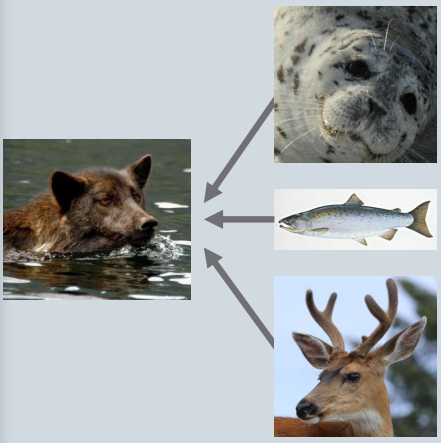
\includegraphics[width=0.8\textwidth]{img/preyDiet.PNG}
\caption{Ejemplo dieta en ecología }
\label{fig:preyDiet}
\end{figure}

\clearpage

\subsection{Movimiento en ecología}

Los modelos de mezcla también se utilizan en ecología para estimar movimientos de animales (fuentes = regiones, mezcla =  animales que pueden desplazarse entre regiones). Estos modelos son usados por ecologistas para calcular composiciones de comunidades y la biodiversidad a nivel de sitio terrestre de todo el mundo.

Para más información artículo \emph{``The PREDICTS database: a global database of how local terrestrial biodiversity responds to human impacts''} \cite{biodiversity:2014}.

\begin{figure}[h!] 
\centering
    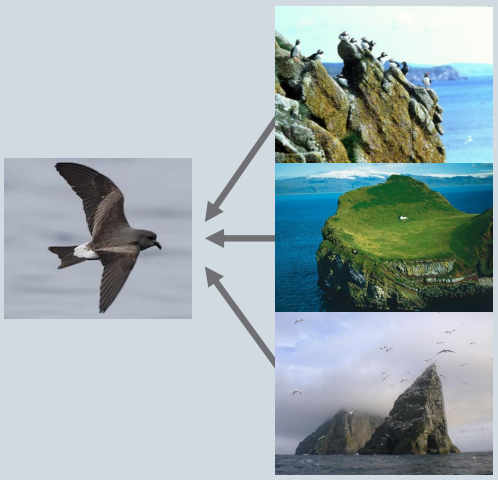
\includegraphics[width=0.8\textwidth]{img/colonyBird.PNG}
\caption{Ejemplo Movimiento en ecología }
\label{fig:colonyBird}
\end{figure}

\clearpage

\subsection{Sedimentos en sistemas fluviales}

Sedimentos en sistemas fluviales (fuentes = terrenos aguas arriba, mezcla = sedimentos aguas abajo). El objetivo de los sistemas de agricultura regenerativa \cite{rodale:1983} es aumentar la calidad del suelo y la biodiversidad de las tierras de labranza, favoreciendo la creación de productos agrícolas nutritivos de forma rentable.

%TODO: \url{https://peerj.com/articles/4428/}
artículo: \url{https://pubmed.ncbi.nlm.nih.gov/30812003/}

\begin{figure}[h!] 
\centering
    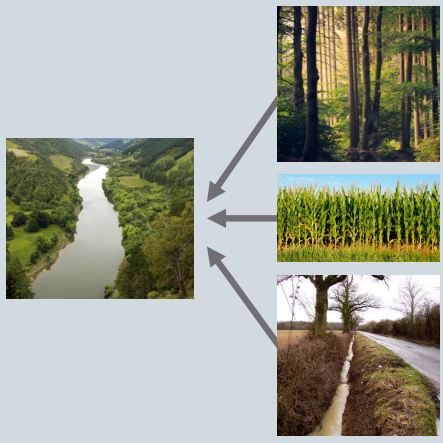
\includegraphics[width=0.8\textwidth]{img/soilSediment.PNG}
\caption{Ejemplo Sedimentos en sistemas fluviales }
\label{fig:soilSediment}
\end{figure}


\clearpage

\section{Cómo funcionan los \emph{Mixing Models}}

Comenzamos explicando un problema sencillo. El problema se plantea dadas dos fuentes posibles de alimentos (Source 1, Source 2) y un consumidor (ver fig. \ref{fig:workMixing0}). Nuestro objetivo es identificar la dieta del consumidor a partir de la composición de sus heces. Para ello, se hace uso de biotrazadores o marcadores, que se encuentran presentes en las fuentes y no se alteran en el proceso de digestión. De esta forma, los biotrazadores nos permiten realizar estimaciones de la cantidad de cada una de las fuentes que puede haber ingerido un consumidor. 

\begin{figure}[h!] 
\centering
    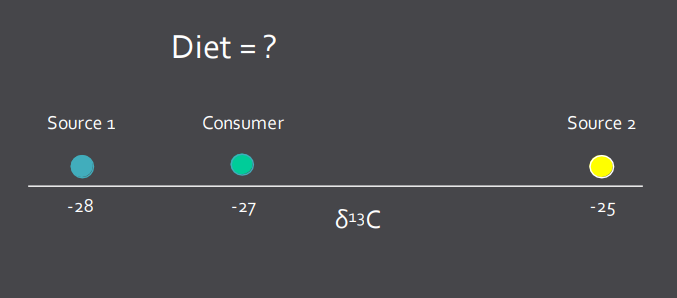
\includegraphics[width=0.8\textwidth]{img/workMixing0.PNG}
\caption{Linear \emph{Mixing Models} - Problema }
\label{fig:workMixing0}
\end{figure}

Para simplificar la explicación supondremos que la masa se conserva durante el proceso de digestión, por ello partimos de la ecuación $p_1 + p_2 = 1$, donde $p_i$ denota la masa de fuente (\emph{source}) $i$ por cada unidad de masa de heces. Como suponemos que la masa se conerva, la suma de las proporciones de las fuentes es igual a 1. Tenemos también una segunda ecuación que refleja la conservación de la masa del biotrazador \textdelta$_{13}C$ a través del proceso de digestión: $Consumer = p_1*S_1 + p_2*S_2$, donde $Consumer$ es la masa de biotrazador en las heces, y $S_i$ denota la concentración de biotrazador en la fuente $i$.

\begin{figure}[h!] 
\centering
    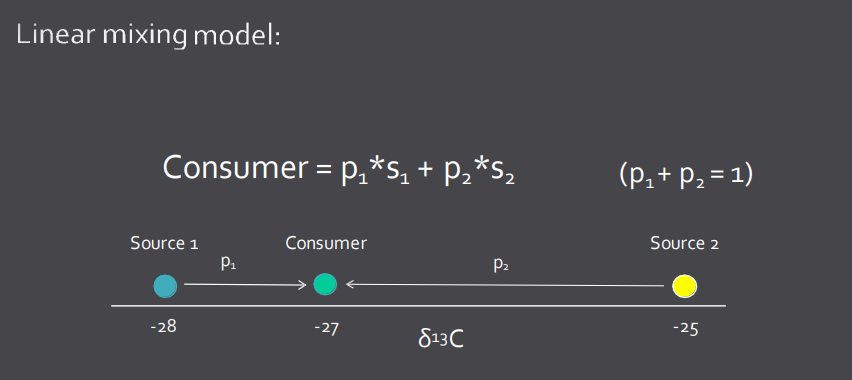
\includegraphics[width=0.8\textwidth]{img/workMixing1.PNG}
\caption{Linear \emph{Mixing Models} - Ecuaciones con un marcador }
\label{fig:workMixing1}
\end{figure}

En el caso de la figura \ref{fig:workMixing1} solo teníamos un eje / biotrazador / marcador, por lo que solo considerábamos una ecuación. En el figura \ref{fig:workMixing2} tenemos dos ejes para los biotrazadores: \textdelta$_{13}C$ y \textdelta$_{15}N$, además de una fuente más ($S_1$, $S_2$, $S_3$). En consecuencia, podemos usar las siguientes ecuaciones: 

$$ Consumer_C = p_1*S_{1C} + p_2*S_{2C} + p_3*S_{3C} $$
$$ Consumer_N = p_1*S_{1N} + p_2*S_{2N} + p_3*S_{3N} $$
$$ p_1 + p_2 = 1 $$

Siendo $S_{iN}$ la concentración del segundo biotrazador  (\textdelta$_{15}N$) en la fuente $i$,  y ese valor se multiplicara por la proporción de la fuente $i$ que se ha ingerido.

\begin{figure}[h!] 
\centering
    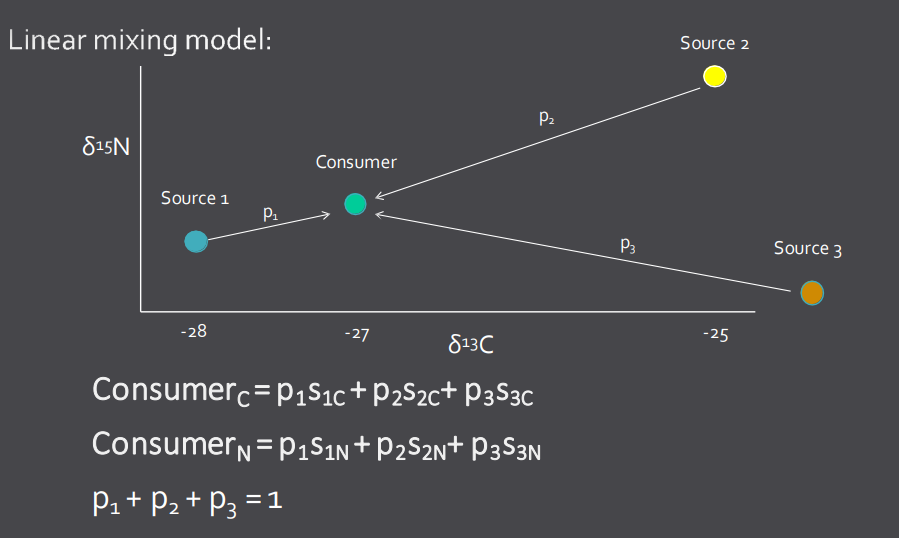
\includegraphics[width=0.8\textwidth]{img/workMixing2.PNG}
\caption{Linear \emph{Mixing Models} - Ecuaciones con dos marcadores }
\label{fig:workMixing2}
\end{figure}

%\subsection{}

En el caso de mi aplicación, se diseñó sin imponer la condición de conservación de la masa. Esto ha ofrecido un mayor realismo a los cálculos de la aplicación, ya que en general la masa de las heces no coincide necesariamente con la suma de las masas que se ingieren (p. ej. los alimentos ingeridos suelen tener más concentración de agua que las heces).

\newpage
\section{Problema n-alcanos}

En esta sección hemos resumido el problema planteado en el artículo \emph{``Using n-alkanes to estimate diet composition of herbivores: a novel mathematical approach''} \cite{problemn-alkanes2007}, que es el punto de partida del proyecto.

Los n-alcanos son hidrocarburos que se encuentran en las cutículas de las plantas, y que pueden ser usados para estimar la composición de la dieta de herbívoros a partir de la composición de sus heces. Conocer la composición de la dieta de los herbívoros es importante para comprender su ecología y alimentación, lo cual es útil para medir sus efectos sobre la vegetación y los ecosistemas.

El modelo usa programación lineal para estimar el mínimo y el máximo de las proporciones de cada planta de la dieta.

Las especies de plantas se caracterizan por diferentes concentraciones de n-alcanos. Los marcadores químicos recuperados en las heces pueden ser utilizados para cuantificar las plantas ingeridas por un animal.
	
Supongamos que $d$ es el número de n-alcanos en planta y hez. Cada hez de la muestra puede ser considerada un \textbf{punto} en el espacio d-Euclideo, que describe la concentración de cada uno de los d n-alcanos. Cada especie de planta puede ser interpretada como un vector en este espacio (Figura \ref{fig:espacio01}).

\begin{figure}[h!] 
\centering
    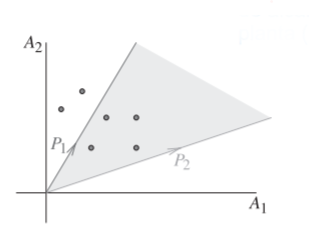
\includegraphics[width=0.4\textwidth]{img/espacio01.png}
\caption{Representación de dos alcanos ($A_1$,$A_2$), dos especies de plantas (vectores $P_1$ y $P_2$), y seis muestras de heces (puntos de la figura). El área sombreada es el cono bidimensional generado por los vectores $P_1$ y $P_2$.}
\label{fig:espacio01}
\end{figure}

Las dietas son combinaciones lineales, es decir, las sumas ponderadas de los vectores que representan las especies vegetales. El peso o coeficiente de cada vector define la cantidad correspondiente de la especie en la dieta. Cada coeficiente dividido  por el sumatorio de los coeficientes, da la proporción de cada planta en la dieta. Si $P_1, P_2, ..., P_p$ son los d-vectores que representan p plantas, cada vector indica la concentración de n-alcanos en esa especie, la combinación lineal con coeficientes $c_1,c_2, ... , c_p$ es $c_1 P_1 + c_2 P_2 + ... + c_p P_p$. \\
Las combinaciones lineales con coeficientes negativos son \textit{"dietas sin sentido"}. Por lo tanto, debemos centrar nuestra atención en las combinaciones lineales que tienen coeficientes no negativos. Este conjunto de combinaciones lineales no negativas forma el cono generado por esos dos vectores. En la Figura \ref{fig:espacio01} el cono generado por los vectores $P_1$ y $P_2$ es la región sombreada. Usamos $C$ para denotar el cono generado, es decir: $$ C = { c_1 P_1 + c_2 P_2 + ... + c_p P_p, \text{ con } c_1,c_2,...,c_p >=0} $$

La estimación de dietas a partir de pruebas fecales $F_1, F_2, ... . F_q $ toma una muestra $F$ y busca sí:

\begin{enumerate}[(i)]
\item $F$ pertenece al cono $C$ o
\item $F$ es un punto fuera de $C$.
\end{enumerate}

Esto es determinado resolviendo el sistema de ecuaciones linear $$Ax=F.$$

Donde A es una matriz $d \times p$ cuyas columnas son los vectores $P_1, P_2 , ... , P_p$ que representan las plantas. Si todos los componentes de la solución $x$ son no-negativos, estaremos en el caso $_{(I)}$, y $x$ especifica la composición correspondiente de especies en las heces. Si hay un componente negativo, estamos en la situación $_{(II)}$, indicando que son \textit{"dietas sin sentido"}. Esto puede resultar de errores en la medición de las concentraciones de n-alcanos, o la existencia de plantas no incluidas en la muestra. Una posible solución es encontrar un vector no negativo de coeficientes que se aproximen a la $x$. Un posible enfoque consiste en:

\begin{enumerate}[(i)]
\setcounter{enumi}{2}
\item identificar un punto $F_0$ en el cono $C$ considerado \textit{"similar a"} $F$, y
\item usando $F_0$ en lugar de $F$, proceder resolviendo como en $_{(I)}$ el sistema de ecuaciones.
\end{enumerate}

Normalmente, la proyección de $F$ en $C$, es decir, el punto en $C$ más cercano a $F$, es seleccionado para ser $F_0$. En la figura \ref{fig:espacio01} hay dos puntos en el caso $_{(II)}$. Cada uno será remplazado por su proyección en $C$, por lo que se encontrará definido por el vector $P_1$.
La dieta estimada del animal se calcula finalmente a partir de las soluciones obtenidas de las muestras fecales $F_1,F_2,...,F_q$.
La dieta son las soluciones del sistema de ecuaciones lineal.

En este ejemplo estamos asumiendo que el número de n-alcanos es igual al número de especies de plantas, es decir, que $A$ es una matriz cuadrada (no-singular). Si hubiera más n-alcanos que especies, la situación no cambiaría (Figura \ref{fig:espacio02}). Pero si hubiese más plantas que n-alcanos (Figura \ref{fig:espacio03}) la situación cambia considerablemente. Ahora cualquier combinación lineal no-negativa de vectores $P_1$ y $P_3$ define un nuevo vector $P$ contenido en el cono generado por estos vectores. Cualquier punto $F$ encontrado en el cono formado por $P$ y $P_2$ es una combinación lineal no negativa de $P$ (en consecuencia de $P$ y $P_3$) y $P_2$. Al ser infinitos los vectores $P$ definidos a partir $P$ y $P_3$ tales que $F$ esta dentro del cono generado en $P$ y $P_2$, el sistema puede tener un número infinito de soluciones no negativas. O lo que es lo mismo, la concentración de n-alcanos en las muestras fecales puede resultar de infinidad de mezclas de plantas diferentes.

\begin{figure}[h!] 
\centering
    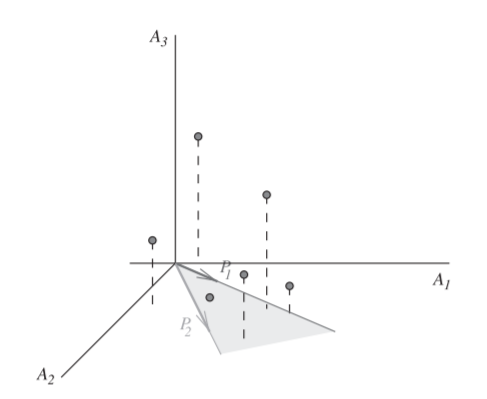
\includegraphics[width=0.4\textwidth]{img/espacio02.png}
\caption{Representación de tres n-alcanos ($A_1$,$A_2$,$A_3$), dos especies de plantas (vectores $P_1$ y $P_2$), y seis muestras de heces (puntos de la figura), dando lugar a un cono bidimensional generado por los dos vectores de plantas.}
\label{fig:espacio02}
\end{figure}

Por tanto, siempre que el número de especies supere al número de n-alcanos se suele enfocar el problema agrupando las especies en categorías. Sin embargo, no existe un claro criterio satisfactorio para decidir cómo agrupar las especies (cómo definir una partición $d$ al conjunto de vectores $P_1, P_2,...,P_p$) ni cómo ponderarlas dentro de cada grupo.

Para resolver este problema se sugiere un enfoque alternativo que usa números arbitrarios de especies de plantas y n-alcanos.

\begin{figure}[h!] 
\centering
    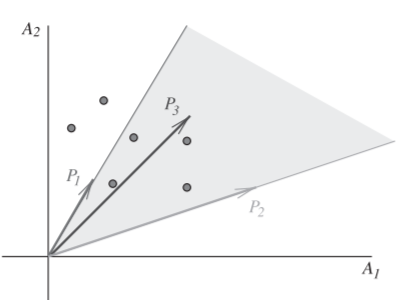
\includegraphics[width=0.4\textwidth]{img/espacio03.png}
\caption{Representación de dos n-alcanos ($A_1$,$A_2$), tres especies de plantas (vectores $P_1$, $P_2$ y $P_3$), y seis muestras de heces (puntos de la figura). El área sombreada es el cono bidimensional generado por los vectores $P_1$, $P_2$ y $P_2$..}
\label{fig:espacio03}
\end{figure}

Partiendo de $P_1, P_2,...,P_p$ vectores de $d$ componentes que representan $p$ plantas, donde $d$ es el número de n-alcanos usados, y $C$ el cono generado por los vectores, denotamos $F_i = 1,2,...,q$ la proyección en $C$ del punto en $d$, y definimos $\phi$ como el conjunto de muestras fecales \textit{``correctas''}.

Definimos una dieta factible, aquella solución no negativa del sistema lineal $Ax=F$, para cualquier punto de $F$ en $\phi$, donde $A$ es $d \times p$ matriz con columnas $P_1, P_2,...,P_p$. Hay muchas dietas factibles. No obstante, el conjunto de dietas está acotado por \textbf{límites superiores e inferiores} para cada uno de los coeficientes, la programación lineal es una herramienta adecuada para abordar algunas de las siguientes cuestiones sobre la dieta:

\begin{itemize}
    \item ¿Cuáles son las proporciones máximas y mínimas de cada especie en la dieta?
    \item ¿Cuáles son las proporciones máximas y mínimas de cada grupo en la dieta?
    \item ¿Cuál es la proporción mínima de una planta, en concreto  en aquellas dietas que cumplen un requisito (por ejemplo, los niveles de ingesta de nitrógeno o tanino contenido)?
\end{itemize}



